\documentclass[Bachelorarbeit.tex]{subfiles}
\begin{document}

\graphicspath{{./figures/appendixResults/}}	%specifying the folder for the figures

\chapter{Results for Hub-Based, Scale-Free and Small-World Topologies}
\label{app:results}

\section{Half-Fully Connected}
\begin{figure}[H]
	\centering
  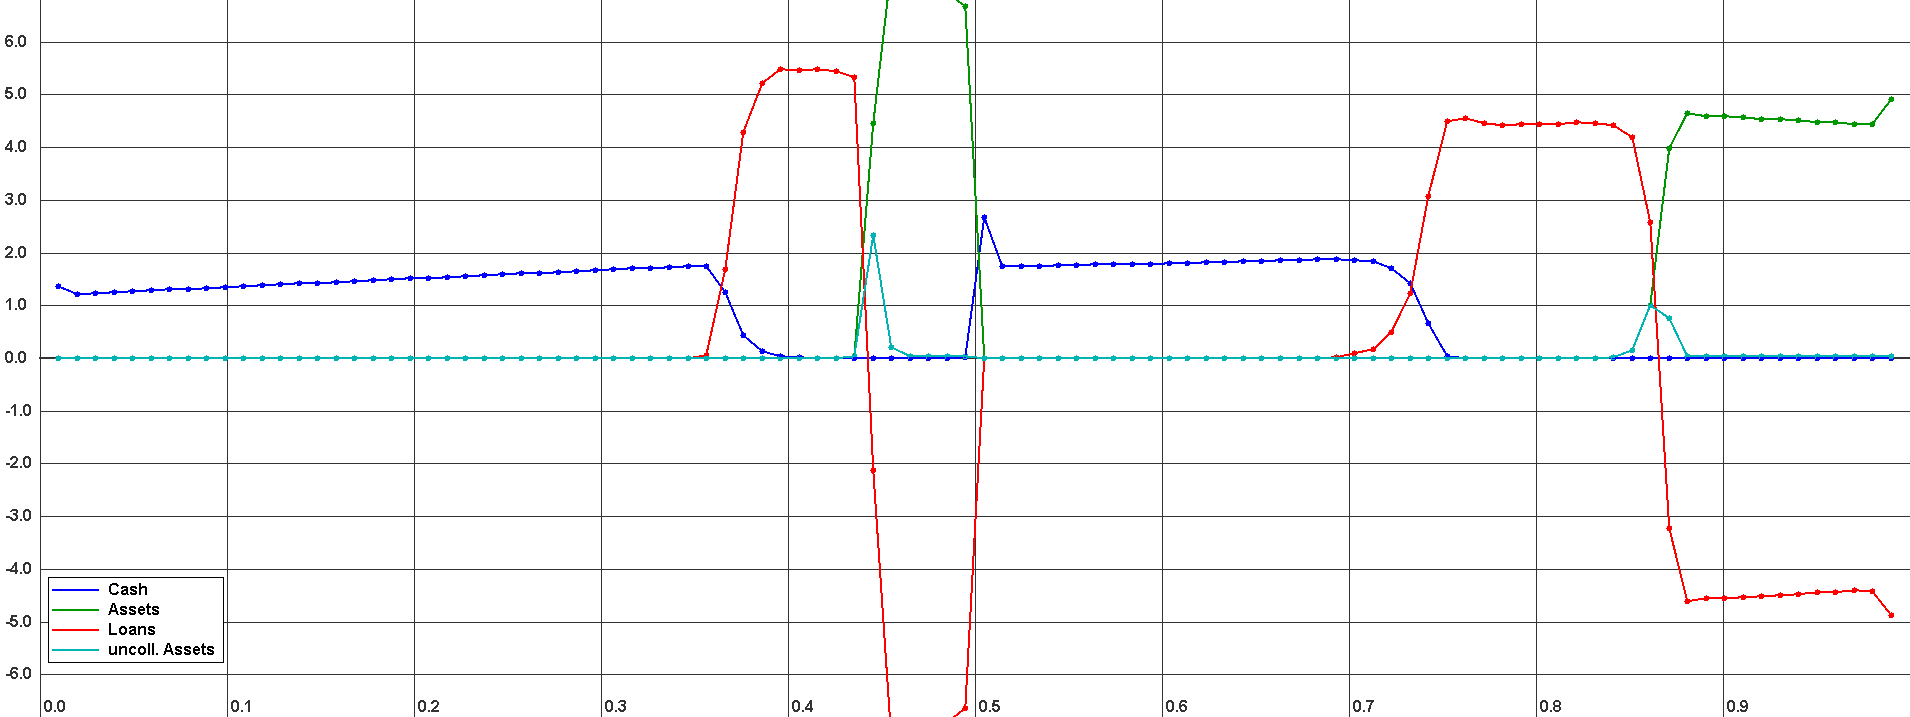
\includegraphics[width=1.0\textwidth, angle=0]{HALFFULLYCONNECTED_100_NOCOLLATERALMARKET_REPL.png}
	\caption{Wealth-Distribution of Half-Fully Connected topology }
	\label{fig:wealth_HALFFULLYCONNECTED_100_NOCOLLATERALMARKET_REPL}
\end{figure}

\begin{table}[H]
	\caption{Equilibrium of Half-Fully Connected topology}
	\centering
	\begin{tabular} { l c r }
		\hline
		Asset-Price p & 0.651 (0.027) \\
		Loan-Price q & 0.362 (0.013) \\
		Marginal Buyer i0 & 0.640 (0.015) \\
		Marginal Seller i1 & 0.833 (0.09) \\
		\hline
		Pessimist Wealth & 1.22 (0.096) \\
		Medianist Wealth & 2.258 (0.409) \\
		Optimist Wealth & 4.526 (0.071) \\
		\hline
	\end{tabular}
\end{table} 

\begin{table}[H]
	\caption{Performance of Half-Fully Connected topology}
	\centering
	\begin{tabular} { l c r }
		\hline
		Successful TX & 14,218.9 (4621.74) \\
		Total TX & 15,253.02 (4633.44) \\
		Failed TX & 1034.12 (22.99) \\
		\hline
	\end{tabular}
\end{table}

\section{Ascending-Connected with short-cuts}

\subsection{Random short-cuts}
\begin{figure}[H]
	\centering
  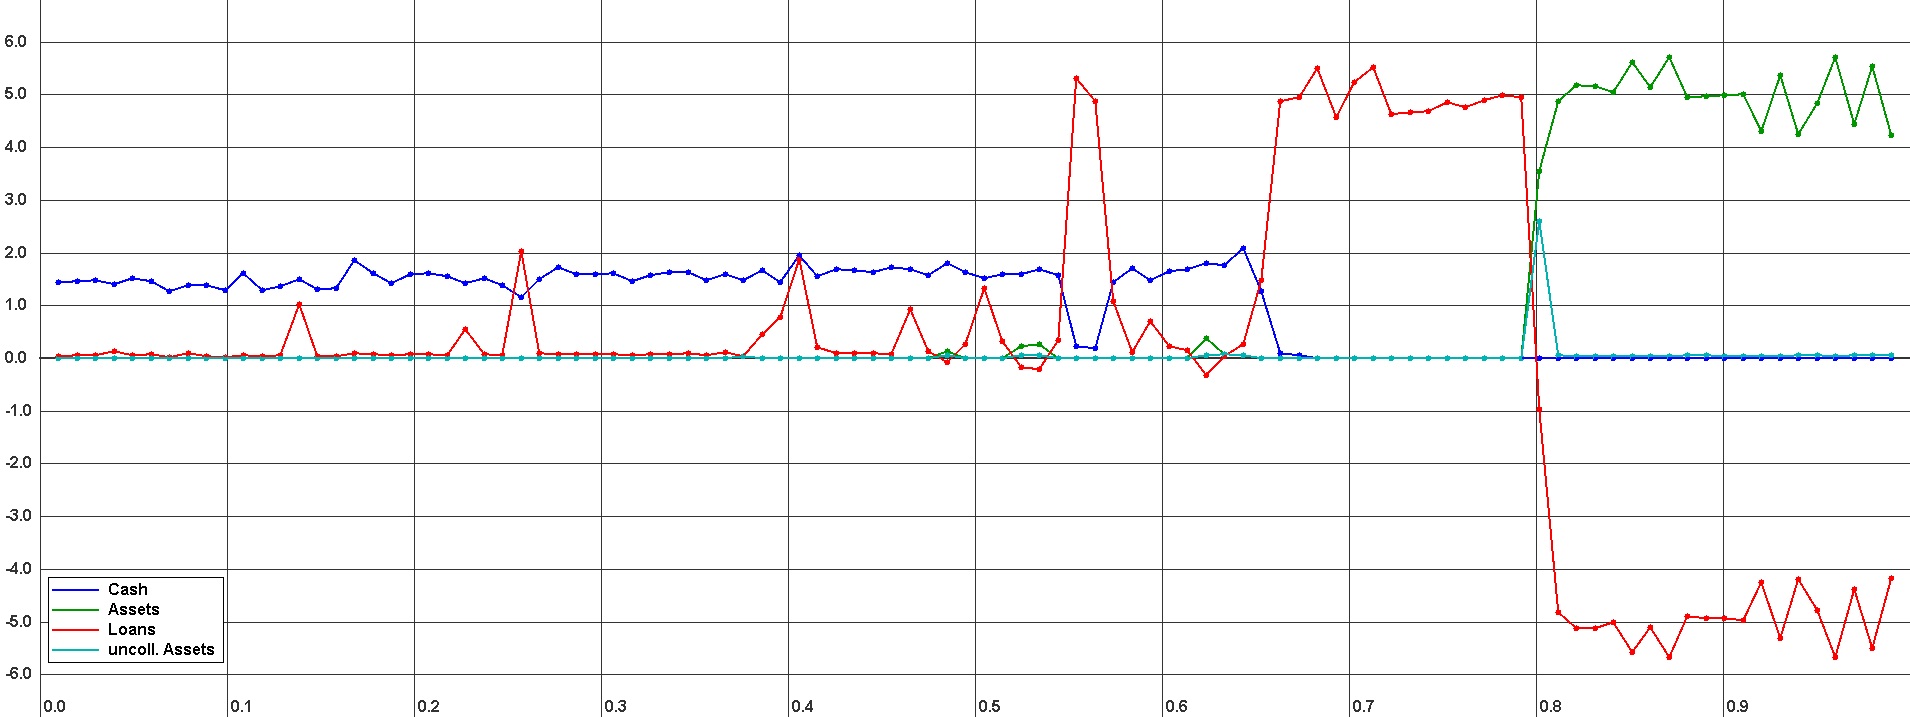
\includegraphics[width=1.0\textwidth, angle=0]{ASCENDINGCONNECTED_RANDSHORTCUTS_100_NOCOLLATERALMARKET_REPL.png}
	\caption{Wealth-Distribution of Ascending-Connected random short-cuts topology}
	\label{fig:wealth_ASCENDINGCONNECTED_RANDSHORTCUTS_100_NOCOLLATERALMARKET_REPL}
\end{figure}

\begin{table}[H]
	\caption{Equilibrium of Ascending-Connected random short-cuts topology}
	\centering
	\begin{tabular} { l c r }
		\hline
		Asset-Price p & 0.731 (0.019) \\
		Loan-Price q & 0.393 (0.009) \\
		Marginal Buyer i0 & 0.649 (0.005) \\
		Marginal Seller i1 & 0.804 (0.004) \\
		\hline
		Pessimist Wealth & 1.441 (0.03) \\
		Medianist Wealth & 4.282 (0.278) \\
		Optimist Wealth & 4.974 (0.038) \\
		\hline
	\end{tabular}
\end{table} 

\begin{table}[H]
	\caption{Performance of Ascending-Connected random short-cuts topology}
	\centering
	\begin{tabular} { l c r }
		\hline
		Successful TX & 8314.78 (229.85) \\
		Total TX & 9496.84 (228.23) \\
		Failed TX & 1182.06 (29.23) \\
		\hline
	\end{tabular}
\end{table}

\subsection{2 short-cuts}
\begin{figure}[H]
	\centering
  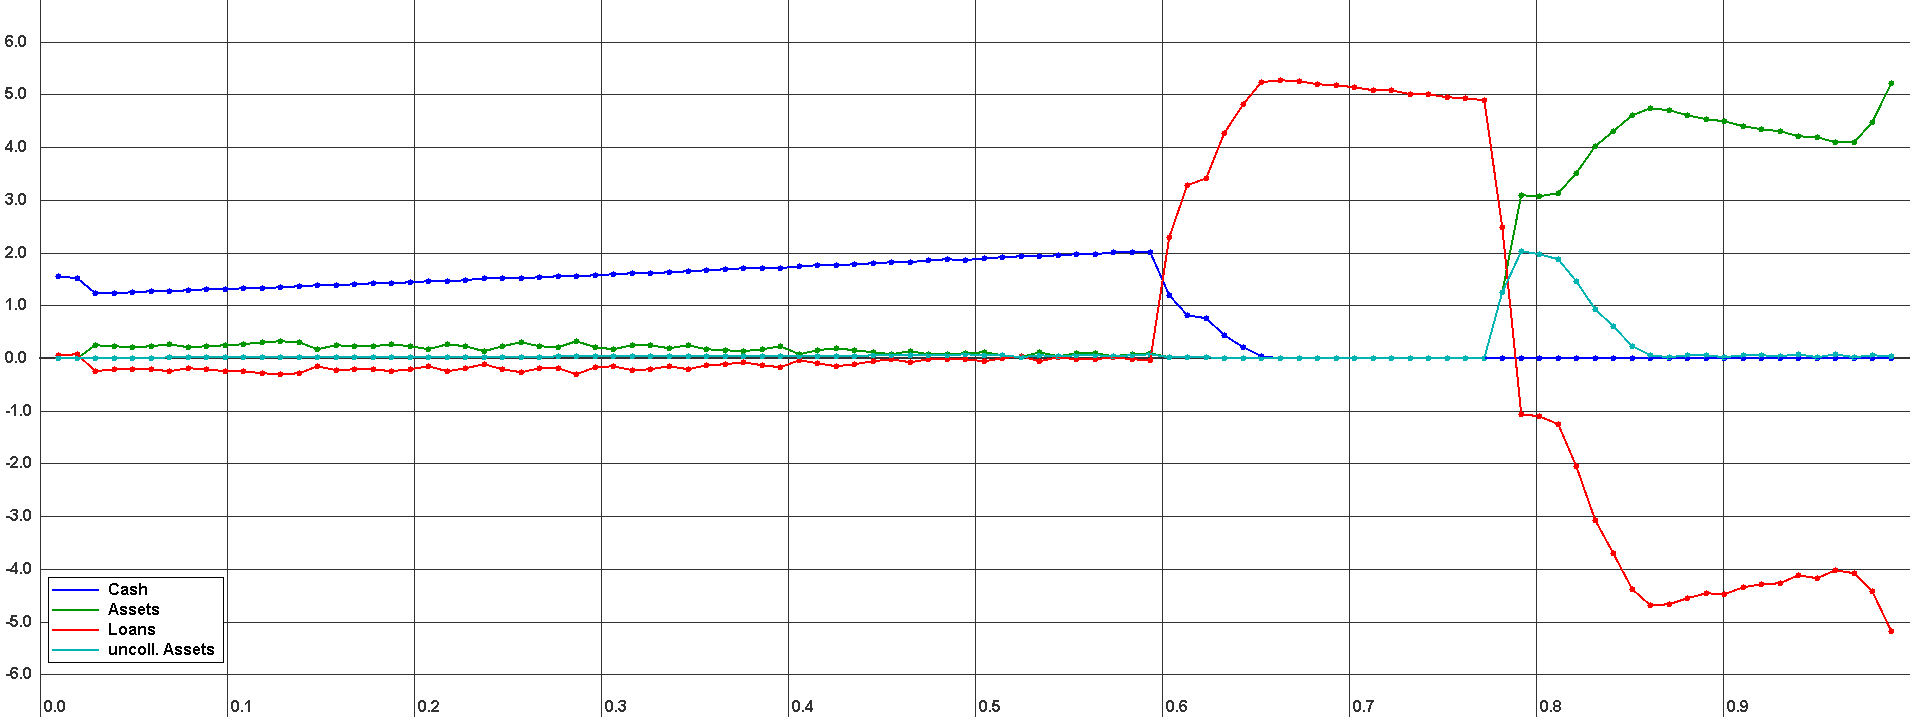
\includegraphics[width=1.0\textwidth, angle=0]{ASCENDINGCONNECTED_2SC_100_NOCOLLATERALMARKET_REPL.png}
	\caption{Wealth-Distribution of Ascending-Connected 2 short-cuts topology}
	\label{fig:wealth_ASCENDINGCONNECTED_2SC_100_NOCOLLATERALMARKET_REPL}
\end{figure}

\begin{table}[H]
	\caption{Equilibrium of Ascending-Connected 2 short-cuts topology}
	\centering
	\begin{tabular} { l c r }
		\hline
		Asset-Price p & 0.662 (0.024) \\
		Loan-Price q & 0.376 (0.006) \\
		Marginal Buyer i0 & 0.608 (0.018) \\
		Marginal Seller i1 & 0.805 (0.028) \\
		\hline
		Pessimist Wealth & 1.441 (0.21) \\
		Medianist Wealth & 3.978 (1.442) \\
		Optimist Wealth & 4.514 (0.063) \\
		\hline
	\end{tabular}
\end{table} 

\begin{table}[H]
	\caption{Performance of Ascending-Connected random short-cuts topology}
	\centering
	\begin{tabular} { l c r }
		\hline
		Successful TX & 37,093.64 (12,864.4) \\
		Total TX & 38,115.54 (12,851.53) \\
		Failed TX & 1021. (18.85) \\
		\hline
	\end{tabular}
\end{table}

\subsection{5 full short-cuts}
\begin{figure}[H]
	\centering
  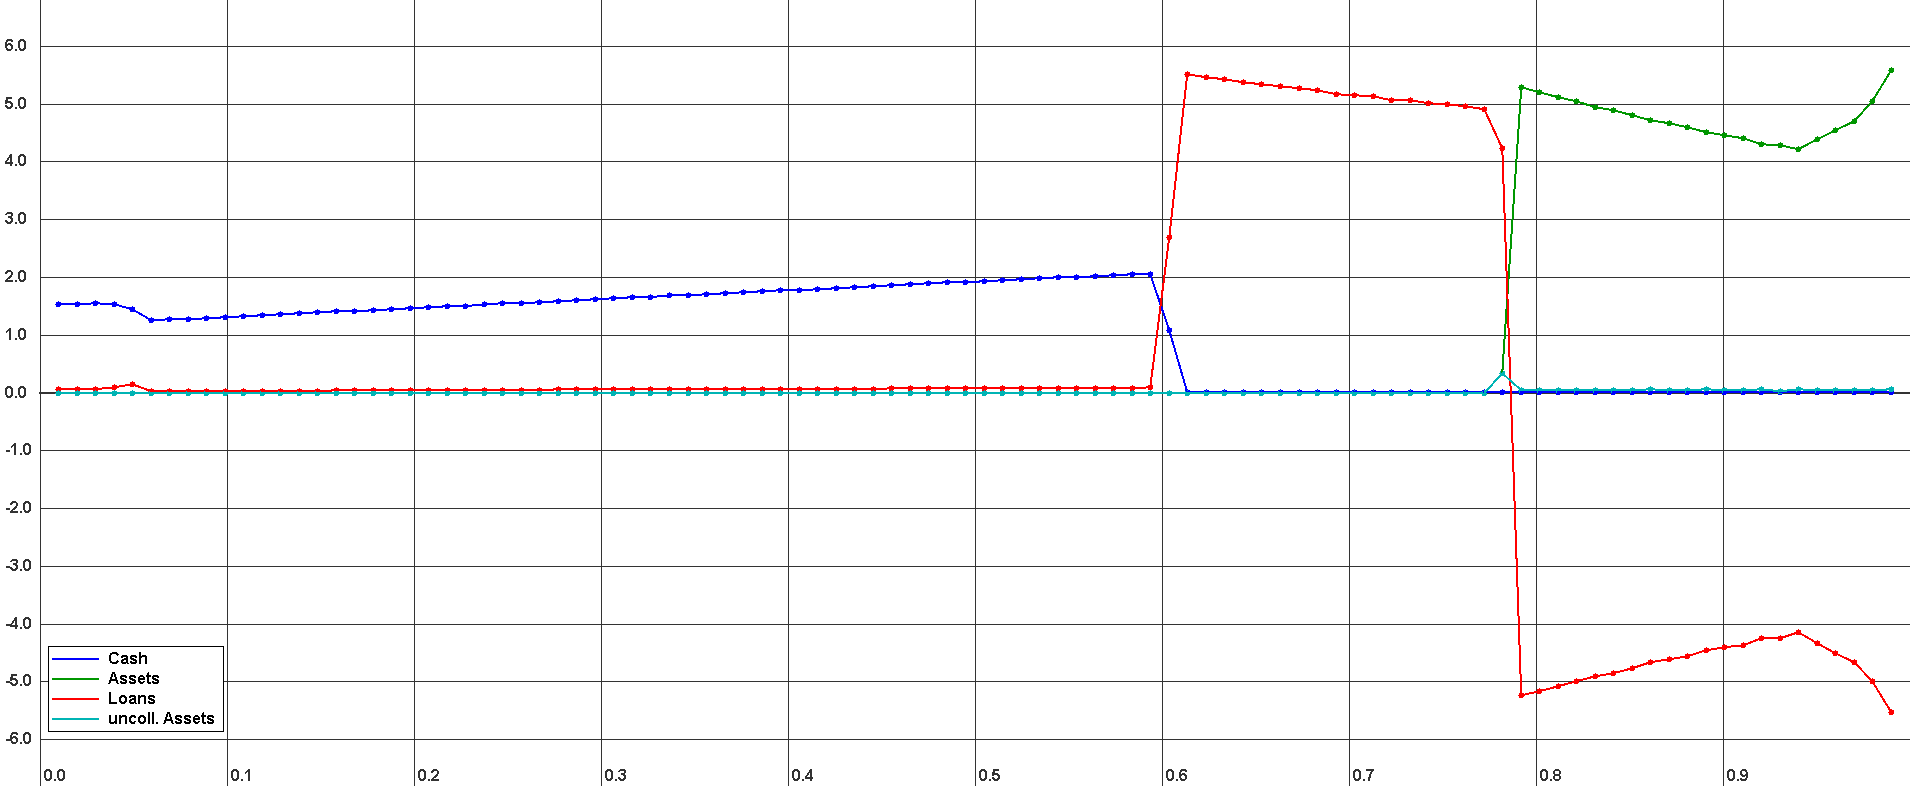
\includegraphics[width=1.0\textwidth, angle=0]{ASCENDINGCONNECTED_5FullSC_100_NOCOLLATERALMARKET_REPL.png}
	\caption{Wealth-Distribution of Ascending-Connected 5 full short-cuts topology}
	\label{fig:wealth_ASCENDINGCONNECTED_5FullSC_100_NOCOLLATERALMARKET_REPL}
\end{figure}

\begin{table}[H]
	\caption{Equilibrium of Ascending-Connected 5 full short-cuts}
	\centering
	\begin{tabular} { l c r }
		\hline
		Asset-Price p & 0.656 (0.019) \\
		Loan-Price q & 0.371 (0.003) \\
		Marginal Buyer i0 & 0.594 (0.0) \\
		Marginal Seller i1 & 0.792 (0.0) \\
		\hline
		Pessimist Wealth & 1.649 (0.002) \\
		Medianist Wealth & 5.013 (0.018) \\
		Optimist Wealth & 4.746 (0.011) \\
		\hline
	\end{tabular}
\end{table} 

\begin{table}[H]
	\caption{Performance of Ascending-Connected 5 full short-cuts topology}
	\centering
	\begin{tabular} { l c r }
		\hline
		Successful TX & 16,971.34 (228.0) \\
		Total TX & 17,998.26 (225.23) \\
		Failed TX & 1026.92 (22.68) \\
		\hline
	\end{tabular}
\end{table}

TODO: move to interpretation: As can be clearly seen 5 full shortcuts seem to be already enough to solve the inefficiencies seen in Ascending-Connected with/without Importance Sampling.

\subsection{15 full short-cuts}
\begin{figure}[H]
	\centering
  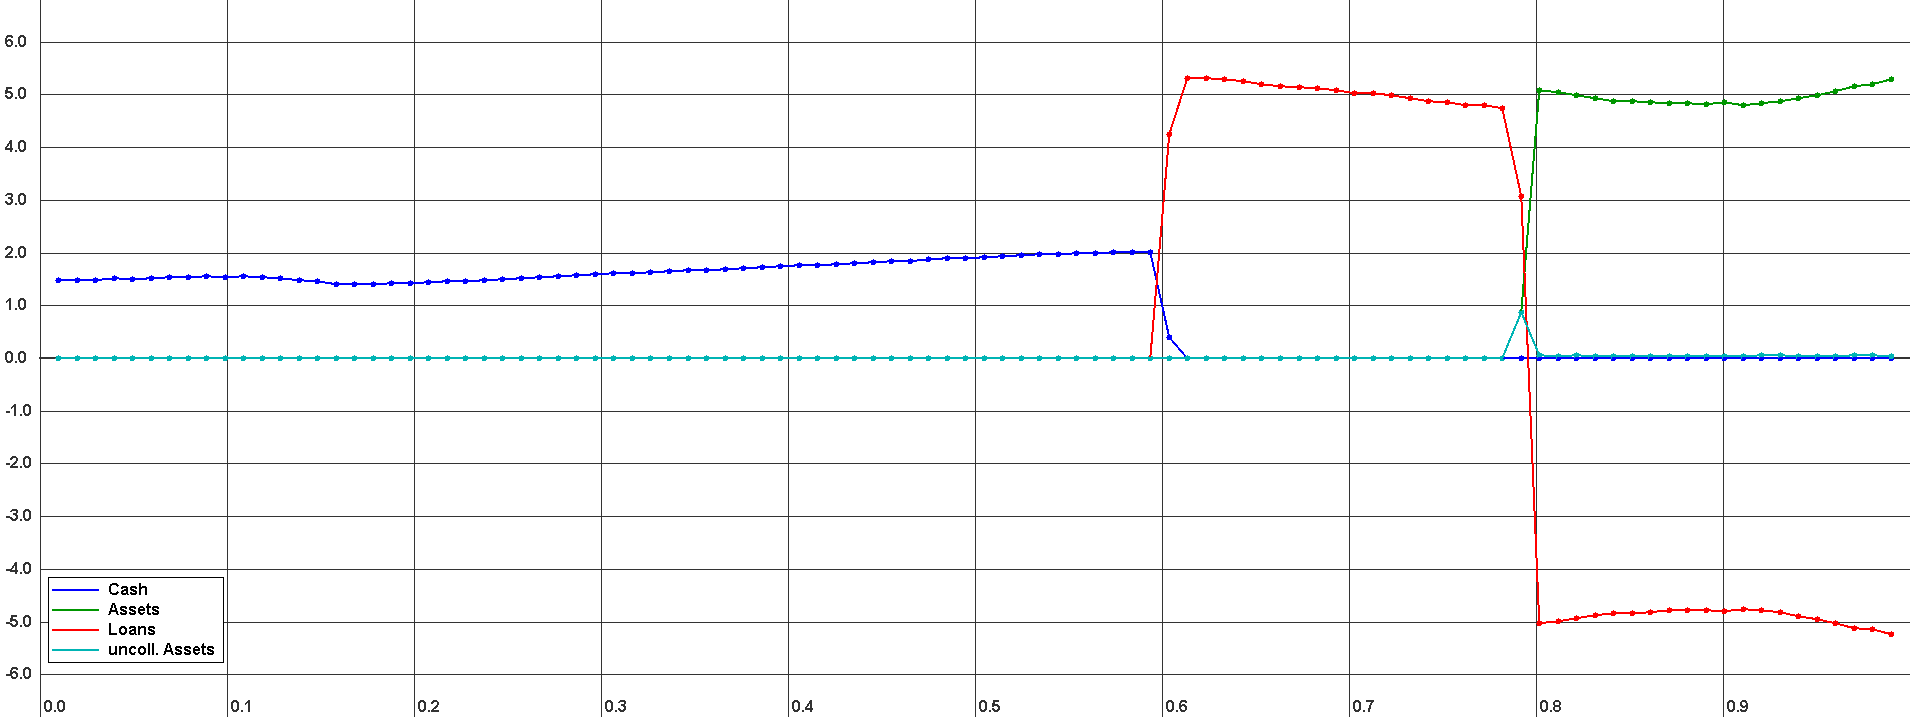
\includegraphics[width=1.0\textwidth, angle=0]{ASCENDINGCONNECTED_15FullSC_100_NOCOLLATERALMARKET_REPL.png}
	\caption{Wealth-Distribution of Ascending-Connected 15 full short-cuts topology}
	\label{fig:wealth_ASCENDINGCONNECTED_15FullSC_100_NOCOLLATERALMARKET_REPL}
\end{figure}

\begin{table}[H]
	\caption{Equilibrium of Ascending-Connected 15 full short-cuts topology}
	\centering
	\begin{tabular} { l c r }
		\hline
		Asset-Price p & 0.658 (0.024) \\
		Loan-Price q & 0.366 (0.009) \\
		Marginal Buyer i0 & 0.601 (0.004) \\
		Marginal Seller i1 & 0.802 (0.0) \\
		\hline
		Pessimist Wealth & 1.649 (0.004) \\
		Medianist Wealth & 4.811 (0.092) \\
		Optimist Wealth & 4.957 (0.021) \\
		\hline
	\end{tabular}
\end{table} 

\begin{table}[H]
	\caption{Performance of Ascending-Connected 15 full short-cuts topology}
	\centering
	\begin{tabular} { l c r }
		\hline
		Successful TX & 4498.08 (58.67) \\
		Total TX & 5522.860 (64.72) \\
		Failed TX & 1024.78 (17.3) \\
		\hline
	\end{tabular}
\end{table}

\subsection{30 full short-cuts}
\begin{figure}[H]
	\centering
  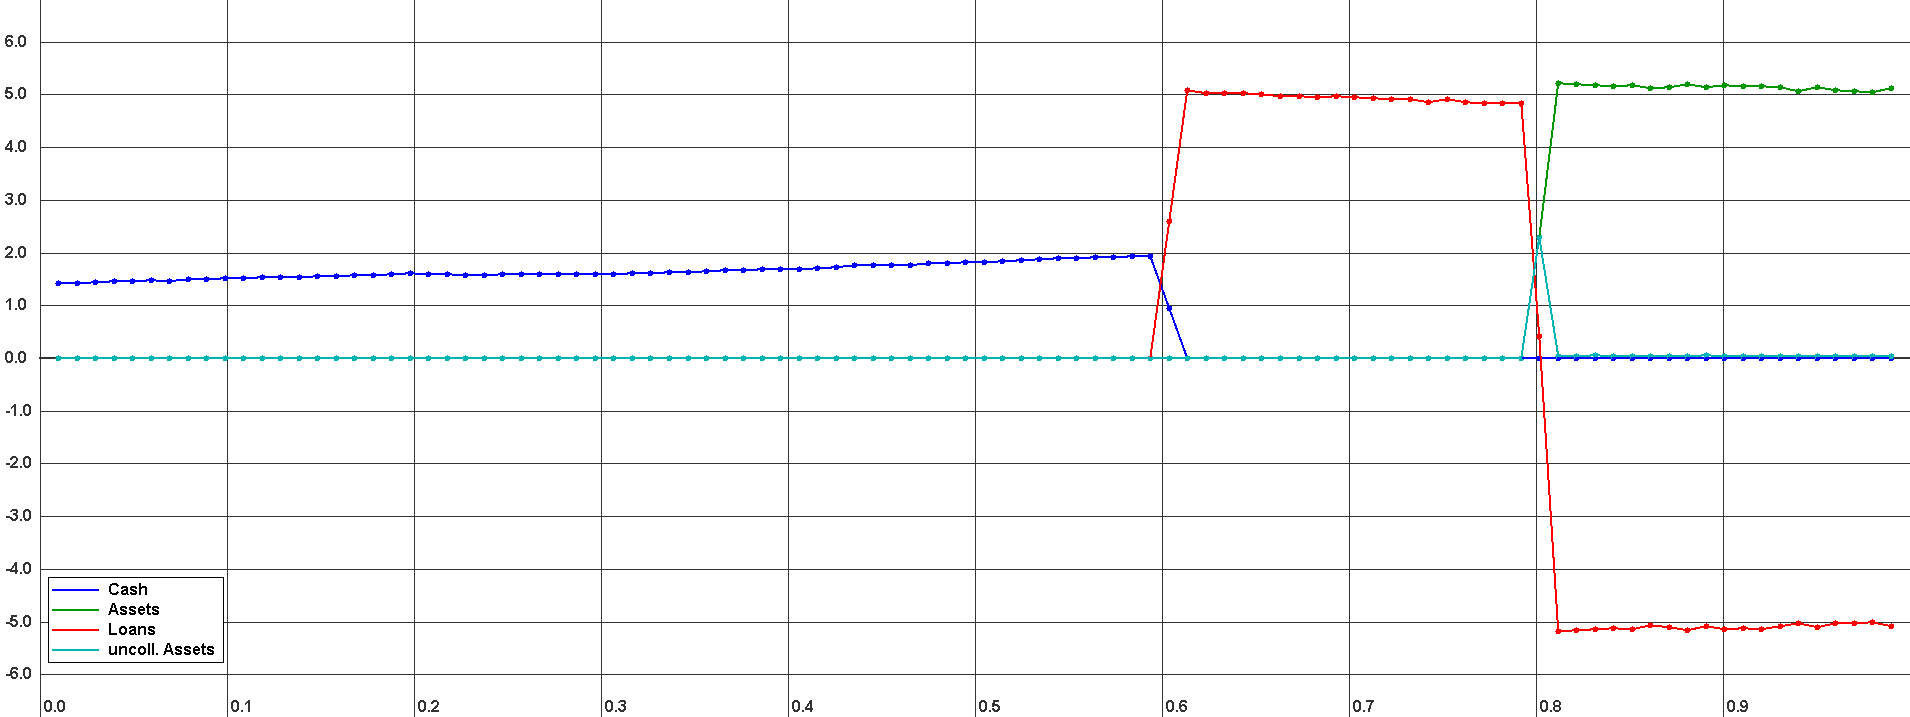
\includegraphics[width=1.0\textwidth, angle=0]{ASCENDINGCONNECTED_30FullSC_100_NOCOLLATERALMARKET_REPL.png}
	\caption{Wealth-Distribution of Ascending-Connected 30 full short-cuts topology}
	\label{fig:wealth_ASCENDINGCONNECTED_30FullSC_100_NOCOLLATERALMARKET_REPL}
\end{figure}

\begin{table}[H]
	\caption{Equilibrium of Ascending-Connected 30 full short-cuts topology}
	\centering
	\begin{tabular} { l c r }
		\hline
		Asset-Price p & 0.681 (0.012) \\
		Loan-Price q & 0.378 (0.006) \\
		Marginal Buyer i0 & 0.603 (0.006) \\
		Marginal Seller i1 & 0.802 (0.1) \\
		\hline
		Pessimist Wealth & 1.649 (0.009) \\
		Medianist Wealth & 4.702 (0.112) \\
		Optimist Wealth & 5.004 (0.025) \\
		\hline
	\end{tabular}
\end{table} 

\begin{table}[H]
	\caption{Performance of Ascending-Connected 30 full short-cuts topology}
	\centering
	\begin{tabular} { l c r }
		\hline
		Successful TX & 2211.08 (35.88) \\
		Total TX & 3225.76 (40.18) \\
		Failed TX & 1014.68 (10.55) \\
		\hline
	\end{tabular}
\end{table}


\subsection{5 regular short-cuts}
\begin{figure}[H]
	\centering
  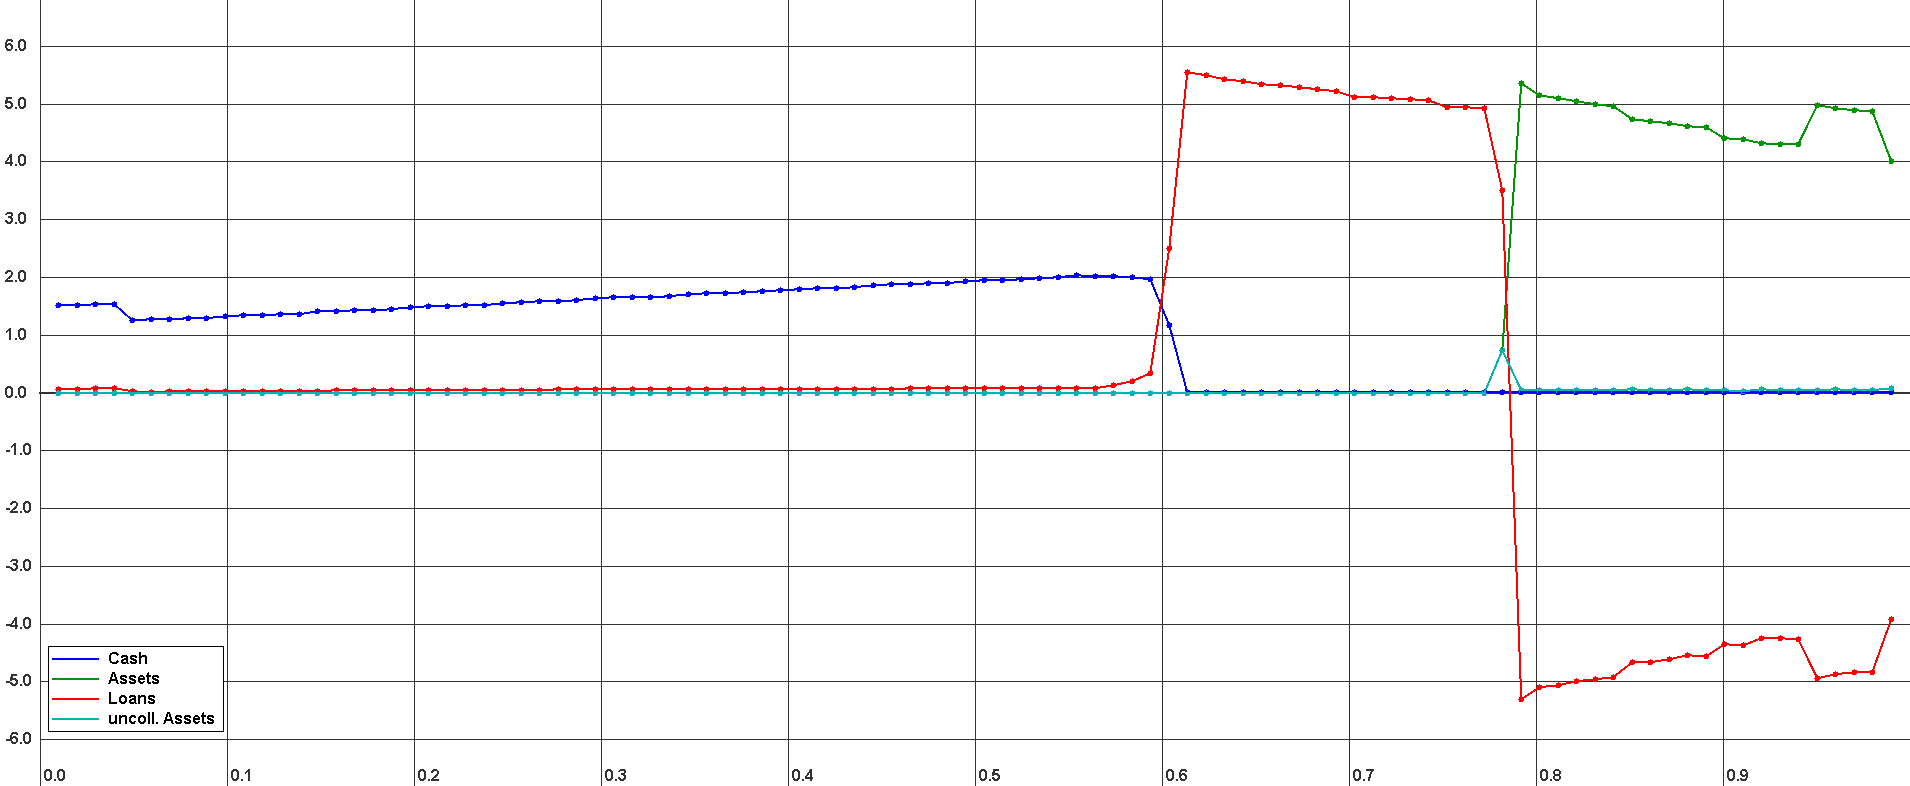
\includegraphics[width=1.0\textwidth, angle=0]{ASCENDINGCONNECTED_5RegSC_100_NOCOLLATERALMARKET_REPL.png}
	\caption{Wealth-Distribution of Ascending-Connected 5 regular short-cuts topology}
	\label{fig:wealth_ASCENDINGCONNECTED_5RegSC_100_NOCOLLATERALMARKET_REPL}
\end{figure}

\begin{table}[H]
	\caption{Equilibrium of Ascending-Connected 5 regular short-cuts topology}
	\centering
	\begin{tabular} { l c r }
		\hline
		Asset-Price p & 0.665 (0.016) \\
		Loan-Price q & 0.364 (0.007) \\
		Marginal Buyer i0 & 0.595 (0.003) \\
		Marginal Seller i1 & 0.792 (0.0) \\
		\hline
		Pessimist Wealth & 1.649 (0.003) \\
		Medianist Wealth & 4.991 (0.045) \\
		Optimist Wealth & 4.727 (0.011) \\
		\hline
	\end{tabular}
\end{table} 

\begin{table}[H]
	\caption{Performance of Ascending-Connected 5 regular short-cuts topology}
	\centering
	\begin{tabular} { l c r }
		\hline
		Successful TX & 14,570.44 (157.61) \\
		Total TX & 15,634.68 (166.21) \\
		Failed TX & 1064.24 (29.88) \\
		\hline
	\end{tabular}
\end{table}

\subsection{15 regular short-cuts}
\begin{figure}[H]
	\centering
  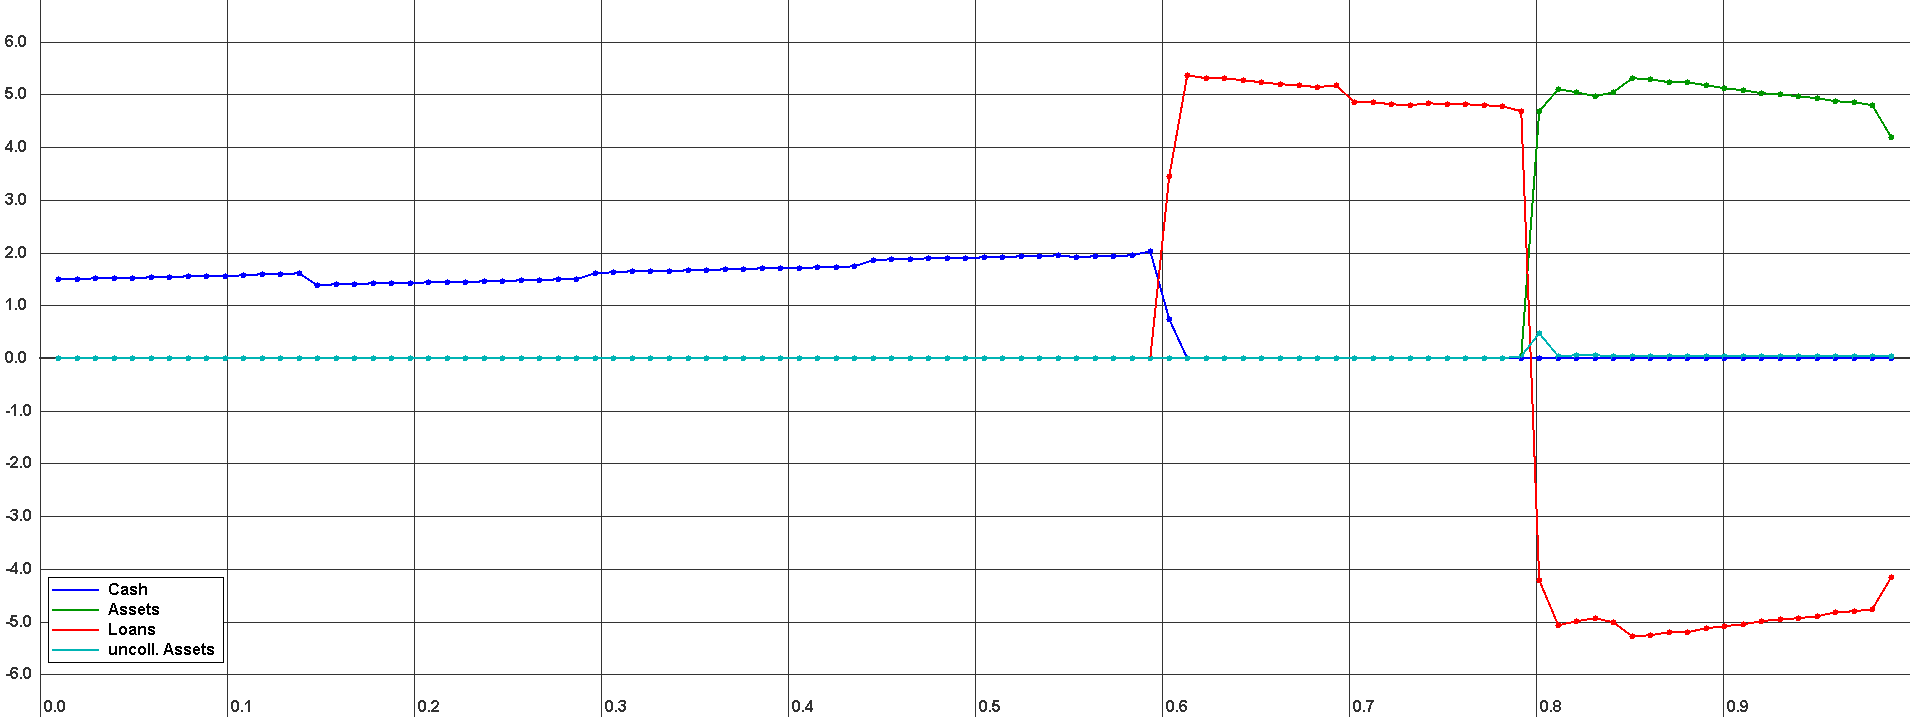
\includegraphics[width=1.0\textwidth, angle=0]{ASCENDINGCONNECTED_15RegSC_100_NOCOLLATERALMARKET_REPL.png}
	\caption{Wealth-Distribution of Ascending-Connected 15 regular short-cuts topology}
	\label{fig:wealth_ASCENDINGCONNECTED_15RegSC_100_NOCOLLATERALMARKET_REPL}
\end{figure}

\begin{table}[H]
	\caption{Equilibrium Ascending-Connected 15 regular short-cuts topology}
	\centering
	\begin{tabular} { l c r }
		\hline
		Asset-Price p & 0.705 (0.020) \\
		Loan-Price q & 0.357 (0.018) \\
		Marginal Buyer i0 & 0.586 (0.023) \\
		Marginal Seller i1 & 0.802 (0.0) \\
		\hline
		Pessimist Wealth & 1.649 (0.051) \\
		Medianist Wealth & 4.146 (0.101) \\
		Optimist Wealth & 4.997 (0.007) \\
		\hline
	\end{tabular}
\end{table} 

\begin{table}[H]
	\caption{Performance of Ascending-Connected 15 regular short-cuts topology}
	\centering
	\begin{tabular} { l c r }
		\hline
		Successful TX & 4373.28 (50.13) \\
		Total TX & 5502.52 (52.11) \\
		Failed TX & 1129.24 (19.2) \\
		\hline
	\end{tabular}
\end{table}

\subsection{30 regular short-cuts}
\begin{figure}[H]
	\centering
  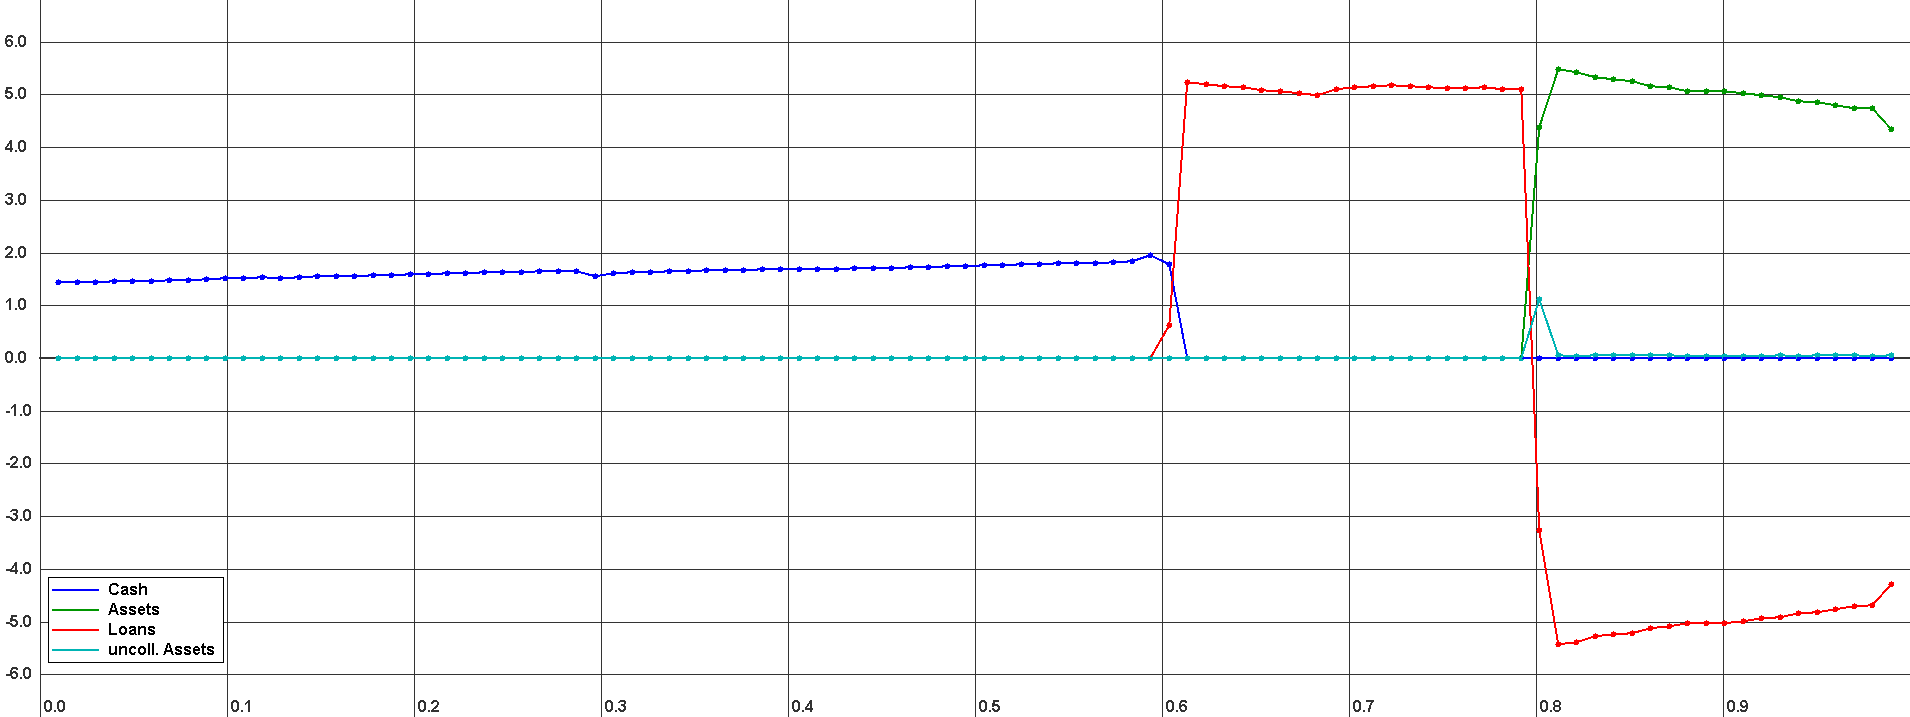
\includegraphics[width=1.0\textwidth, angle=0]{ASCENDINGCONNECTED_30RegSC_100_NOCOLLATERALMARKET_REPL.png}
	\caption{Wealth-Distribution of Ascending-Connected 30 regular short-cuts topology}
	\label{fig:wealth_ASCENDINGCONNECTED_30RegSC_100_NOCOLLATERALMARKET_REPL}
\end{figure}

\begin{table}[H]
	\caption{Equilibrium of Ascending-Connected 30 regular short-cuts topology}
	\centering
	\begin{tabular} { l c r }
		\hline
		Asset-Price p & 0.710 (0.021) \\
		Loan-Price q & 0.398 (0.008) \\
		Marginal Buyer i0 & 0.589 (0.021) \\
		Marginal Seller i1 & 0.802 (0.0) \\
		\hline
		Pessimist Wealth & 1.479 (0.049) \\
		Medianist Wealth & 3.713 (0.125) \\
		Optimist Wealth & 5.0 (0.0) \\
		\hline
	\end{tabular}
\end{table} 

\begin{table}[H]
	\caption{Performance of Ascending-Connected 30 regular short-cuts topology}
	\centering
	\begin{tabular} { l c r }
		\hline
		Successful TX & 5427.02 (90.82) \\
		Total TX & 6566.06 (96.04) \\
		Failed TX & 1139.04 (27.74) \\
		\hline
	\end{tabular}
\end{table}



\section{Hub-Based topologies} 
The Hub-Based Topologies fail to come even close to equilibrium due to reasons given in Chapter "Topologies and Hypothesis". This can be seen also very clearly in the visual results and thus no performance- and equilibrium-tables are listed as they would not make any sense.

\subsection{3-Hubs}
\begin{figure}[H]
	\centering
  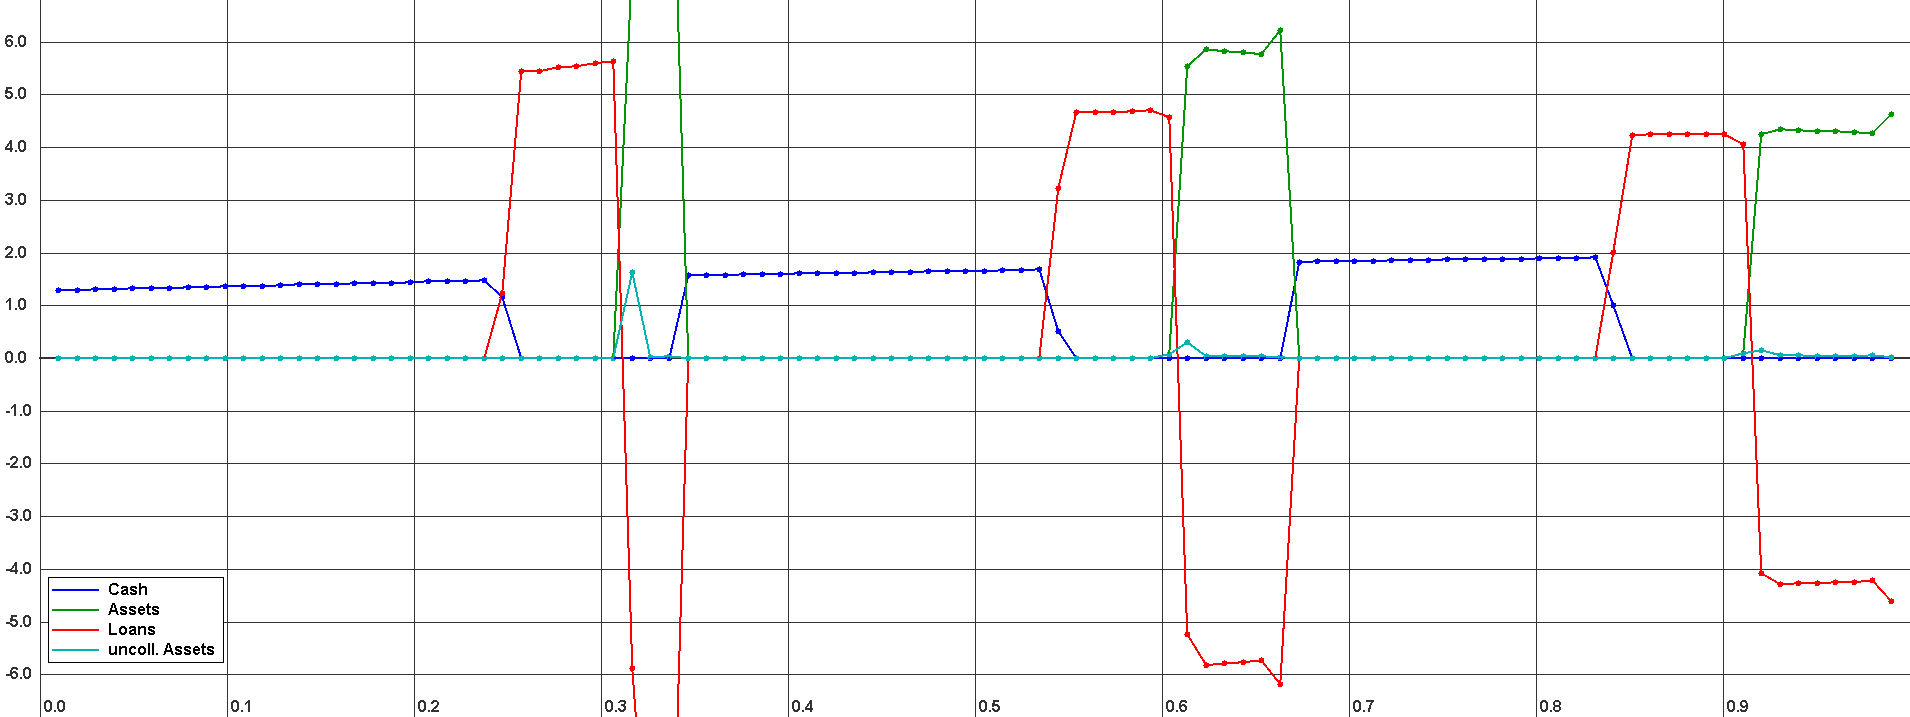
\includegraphics[width=1.0\textwidth, angle=0]{3HUBS_100_NOCOLLATERALMARKET_REPL.png}
	\caption{Wealth-Distribution of 3-Hubs topology}
	\label{fig:wealth_3HUBS_100_NOCOLLATERALMARKET_REPL}
\end{figure}

\subsection{1-Median Hub}
\begin{figure}[H]
	\centering
  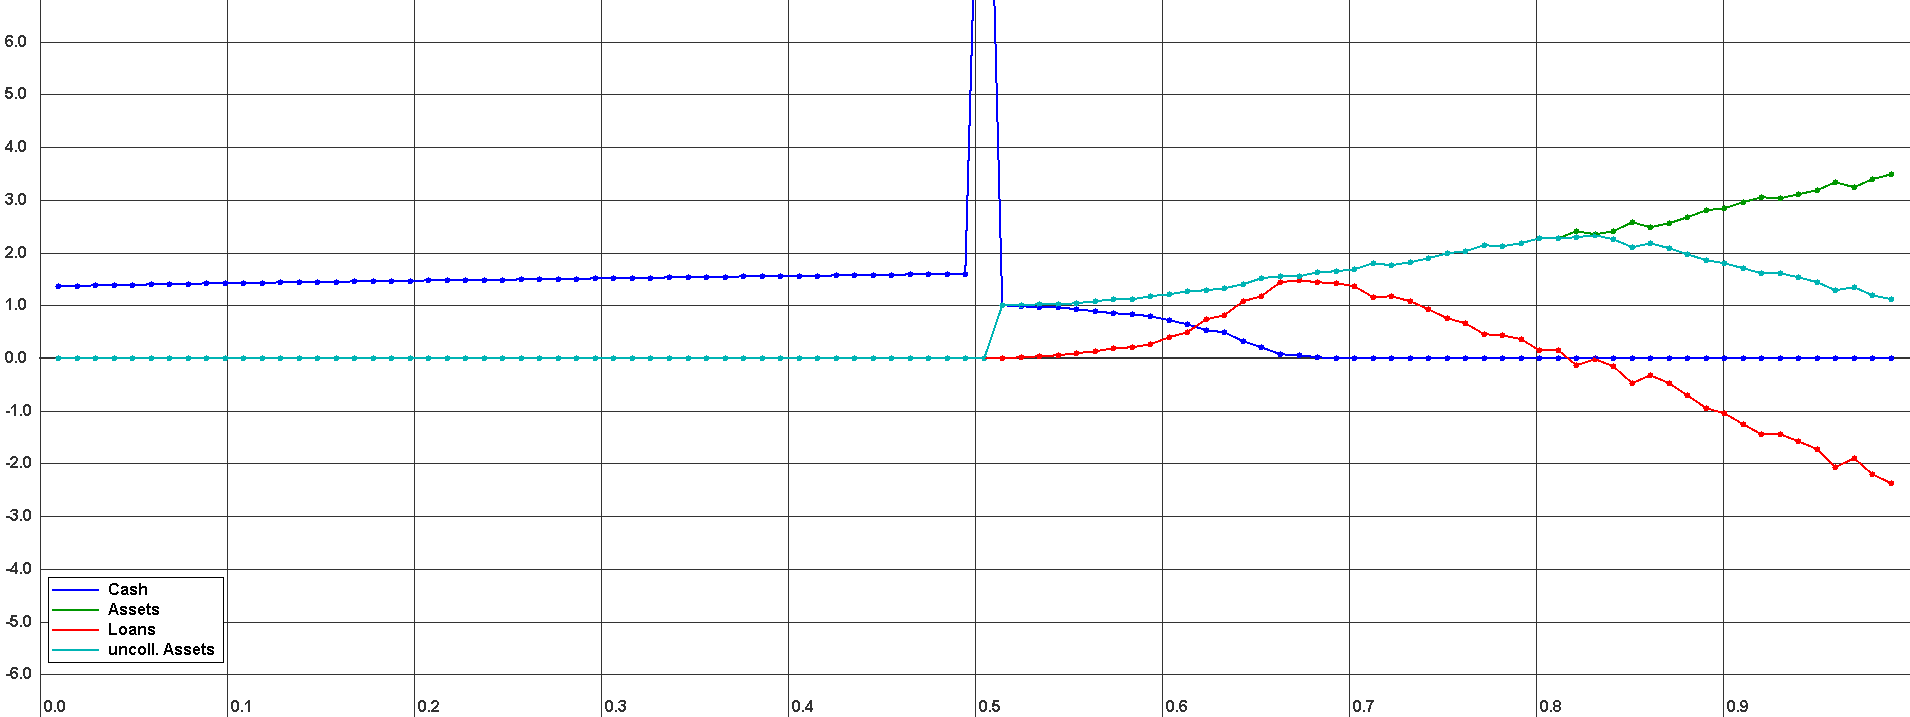
\includegraphics[width=1.0\textwidth, angle=0]{1MEDIANHUB_100_NOCOLLATERALMARKET_REPL.png}
	\caption{Wealth-Distribution of 1 Median-Hub topology}
	\label{fig:wealth_1MEDIANHUB_100_NOCOLLATERALMARKET_REPL}
\end{figure}

\subsection{3-Median Hubs}
\begin{figure}[H]
	\centering
  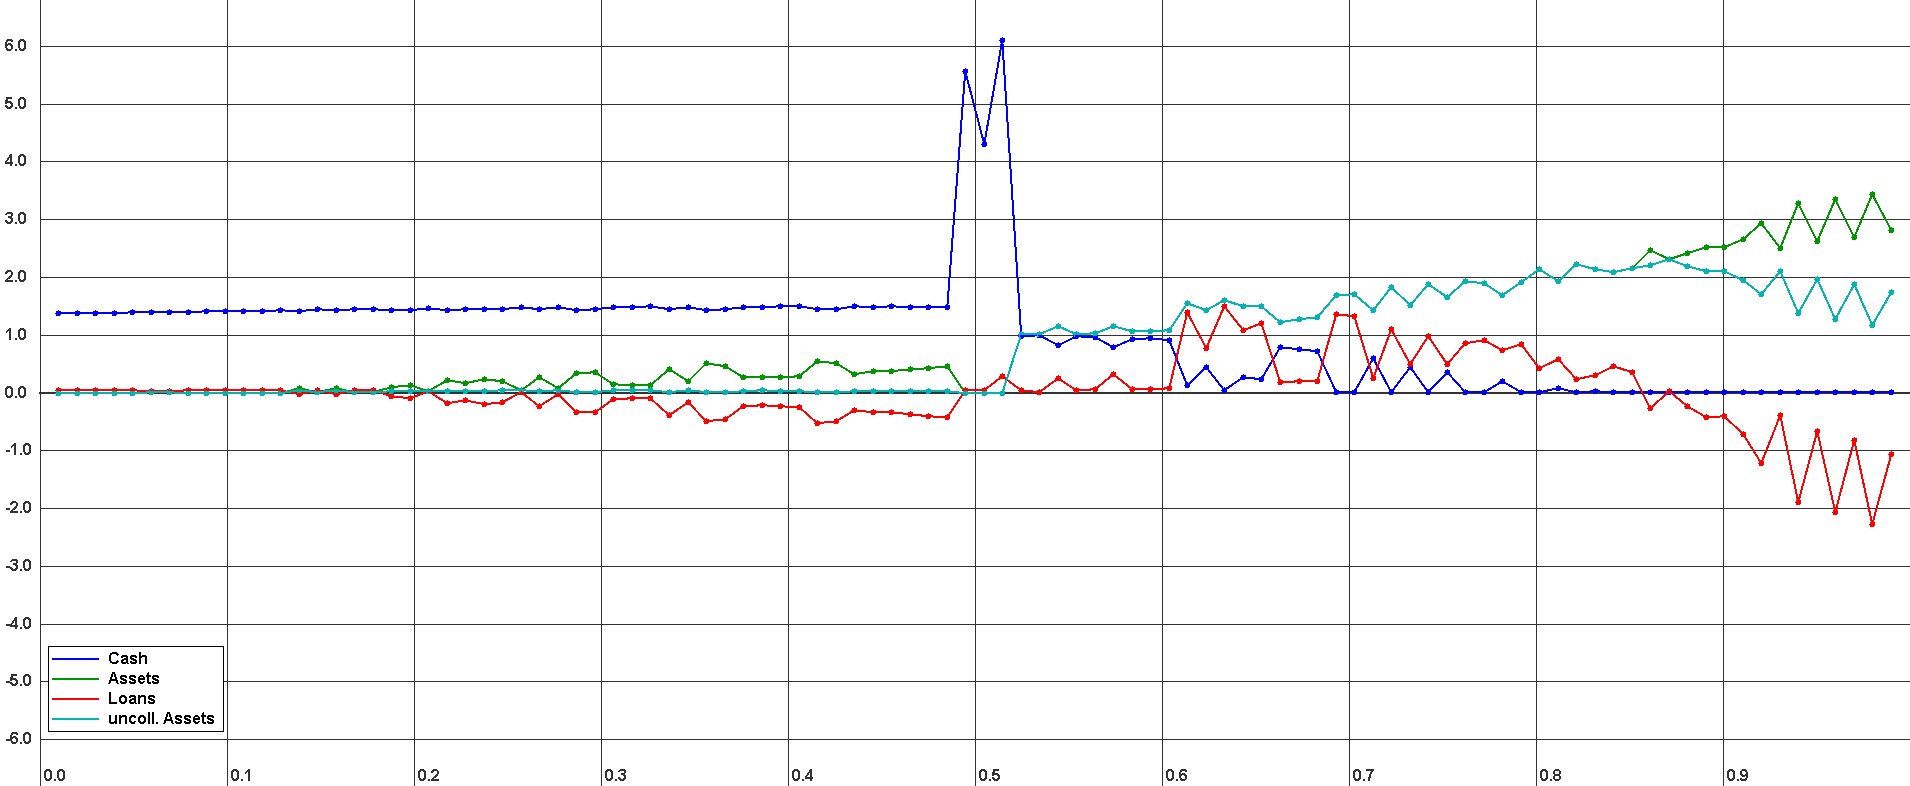
\includegraphics[width=1.0\textwidth, angle=0]{3MEDIANHUBS_100_NOCOLLATERALMARKET_REPL.png}
	\caption{Wealth-Distribution of 3 Median-Hubs topology}
	\label{fig:wealth_3MEDIANHUBS_100_NOCOLLATERALMARKET_REPL}
\end{figure}

\subsection{Maximum Hub}
\begin{figure}[H]
	\centering
  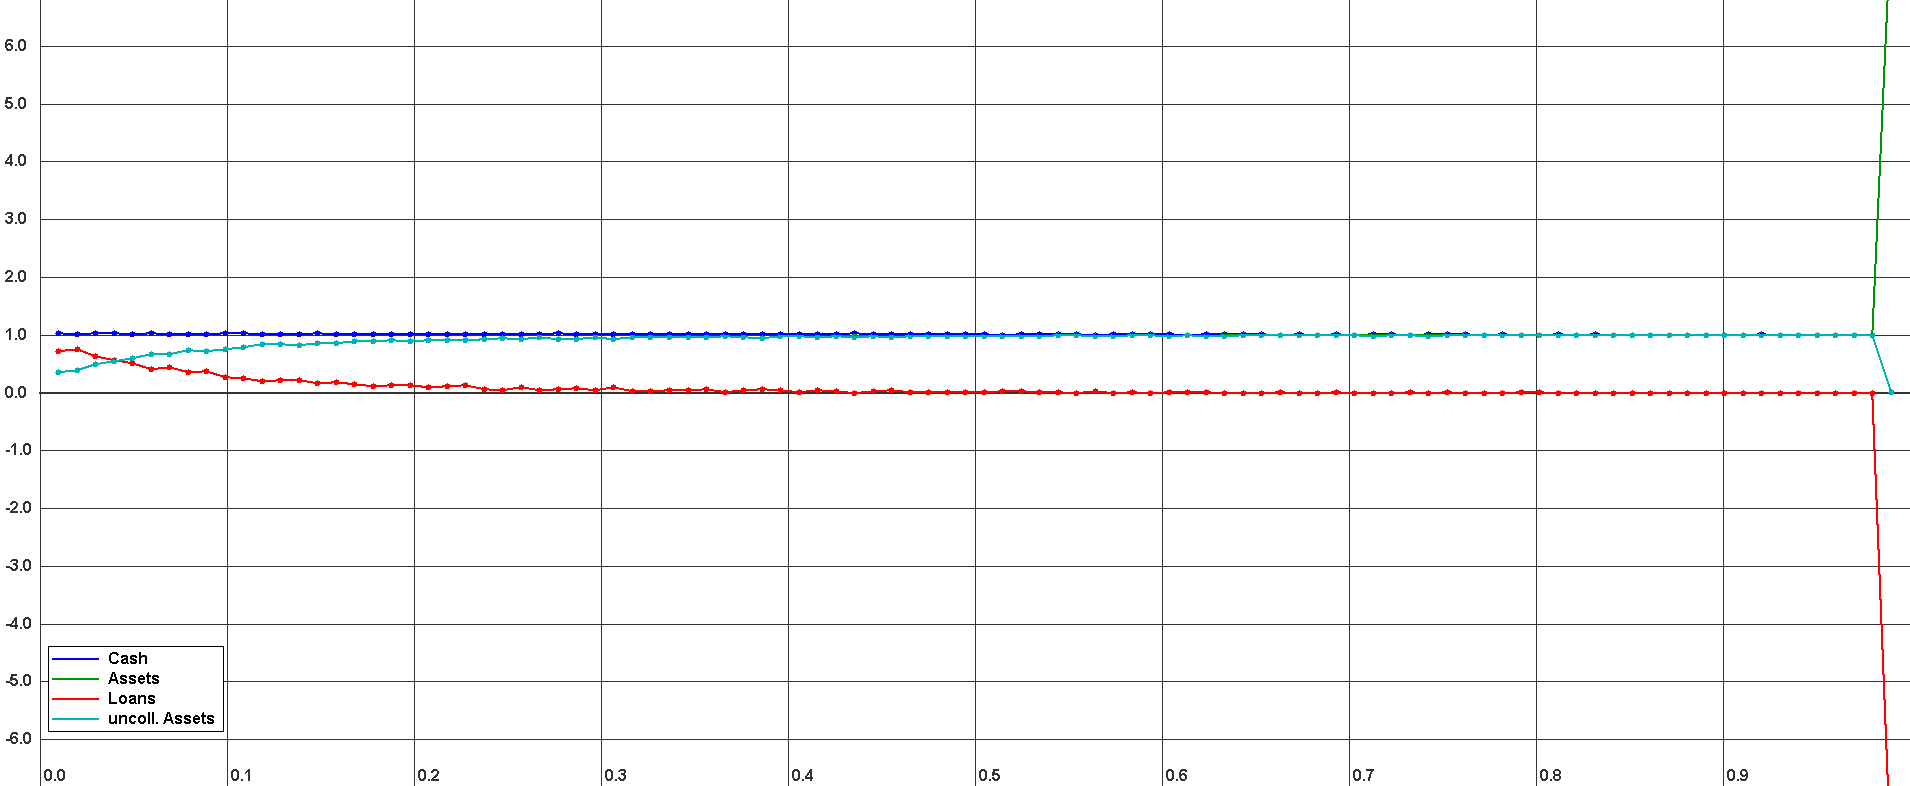
\includegraphics[width=1.0\textwidth, angle=0]{MAXIMUMHUB_100_NOCOLLATERALMARKET_REPL.png}
	\caption{Wealth-Distribution of Maximum-Hub topology}
	\label{fig:wealth_MAXIMUMHUB_100_NOCOLLATERALMARKET_REPL}
\end{figure}

\section{Scale-Free and Small-World topologies}
This topologies fail to come even close to equilibrium too due to reasons given in Chapter "Topologies and Hypothesis". This can be seen also very clearly in the visual results and thus no performance- and equilibrium-tables are listed as they would not make any sense.

\subsection{Erdos-Renyi}
todo: kann hypothese erfüllen mit entsprechender parameterisierung

\begin{figure}[H]
	\centering
  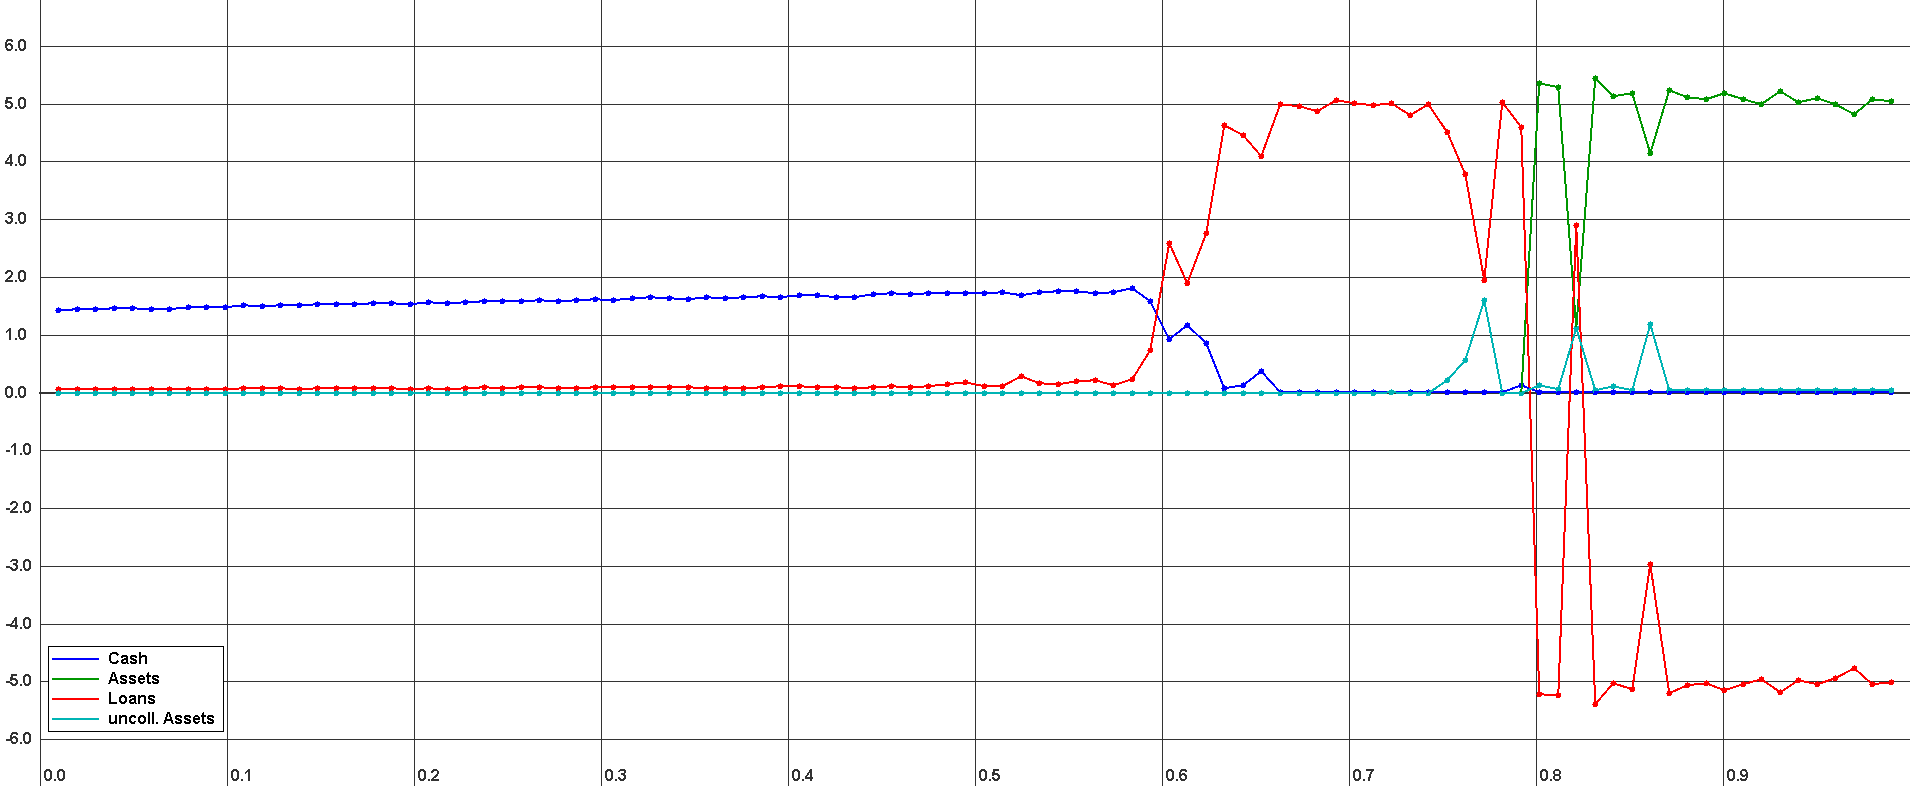
\includegraphics[width=1.0\textwidth, angle=0]{ERDOSRENYI_02_100_NOCOLLATERALMARKET_REPL.png}
	\caption{Wealth-Distribution of Erdos-Renyi 0.2 topology}
	\label{fig:wealth_ERDOSRENYI_02_100_NOCOLLATERALMARKET_REPL}
\end{figure}

need to show network too because random ?

\begin{figure}[H]
	\centering
  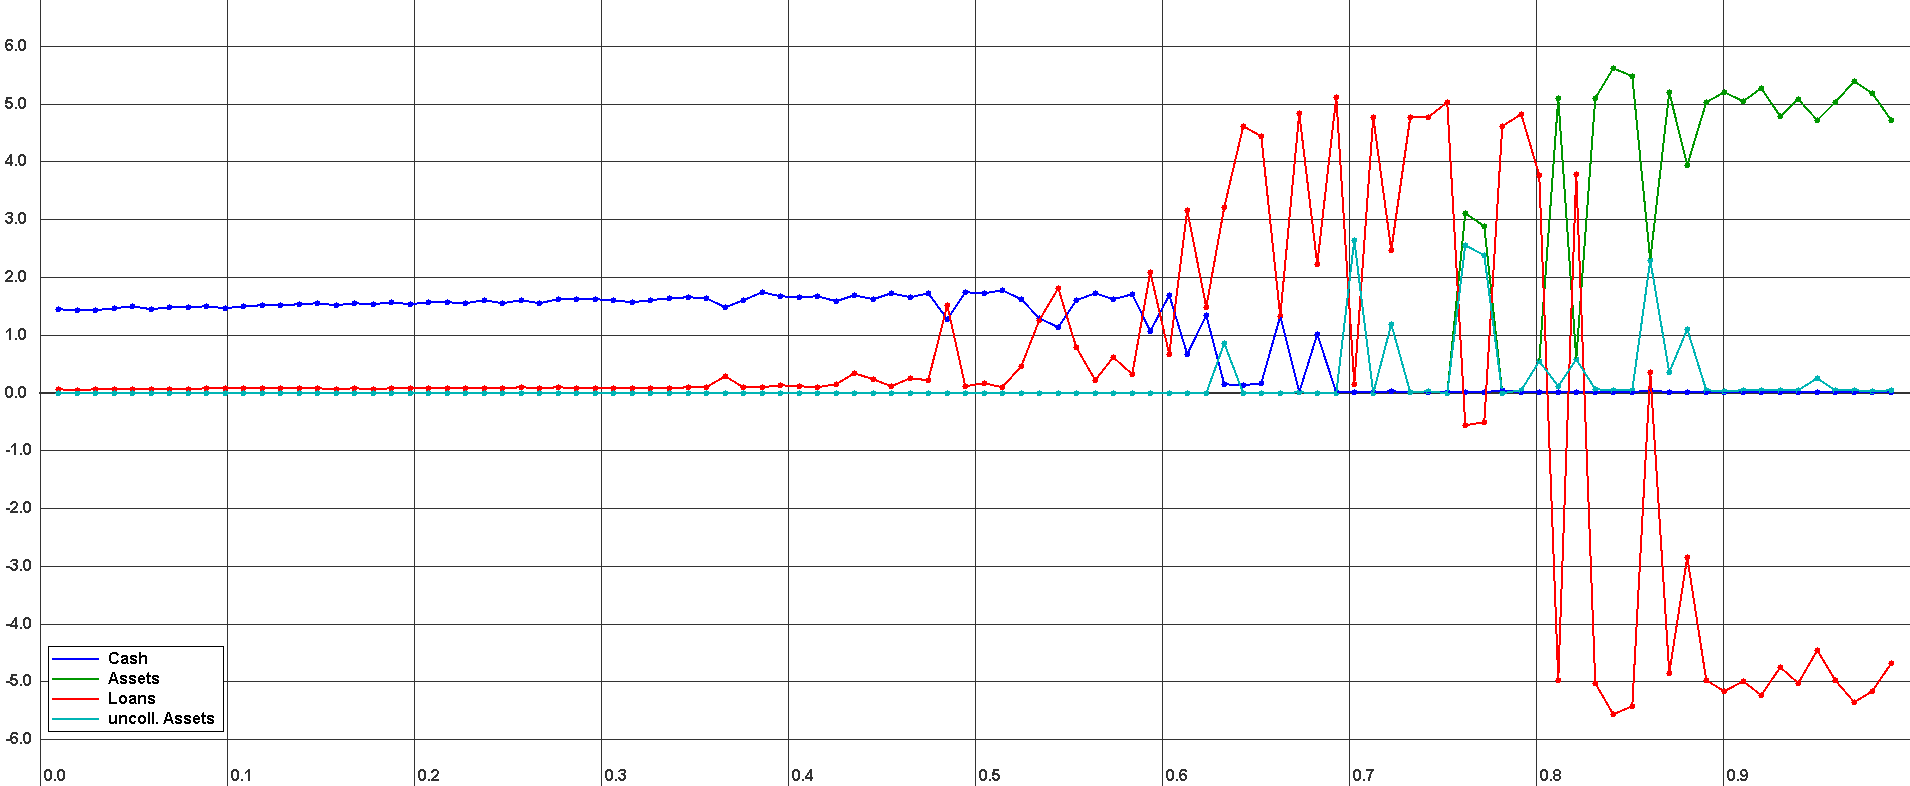
\includegraphics[width=1.0\textwidth, angle=0]{ERDOSRENYI_01_100_NOCOLLATERALMARKET_REPL.png}
	\caption{Wealth-Distribution of Erdos-Renyi 0.1 topology}
	\label{fig:wealth_ERDOSRENYI_01_100_NOCOLLATERALMARKET_REPL}
\end{figure}

need to show network too because random ?

\begin{figure}[H]
	\centering
  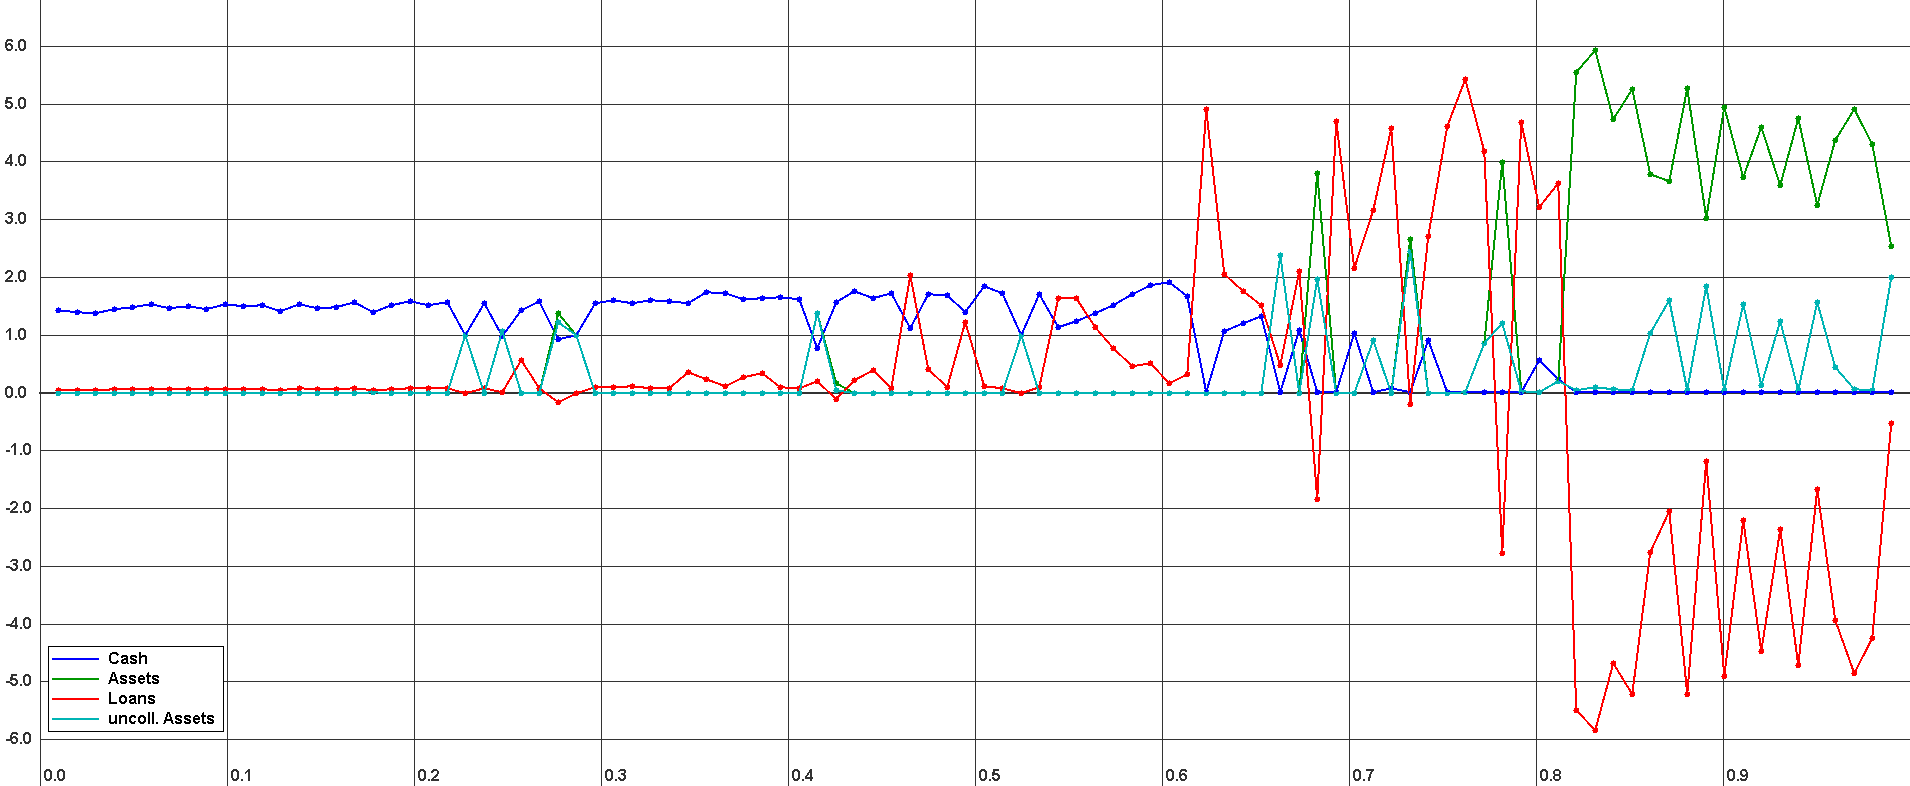
\includegraphics[width=1.0\textwidth, angle=0]{ERDOSRENYI_005_100_NOCOLLATERALMARKET_REPL.png}
	\caption{Wealth-Distribution of Erdos-Renyi 0.05 topology}
	\label{fig:wealth_ERDOSRENYI_005_100_NOCOLLATERALMARKET_REPL}
\end{figure}

need to show network too because random ?

\subsection{Barbasi-Albert}
\begin{figure}[H]
	\centering
  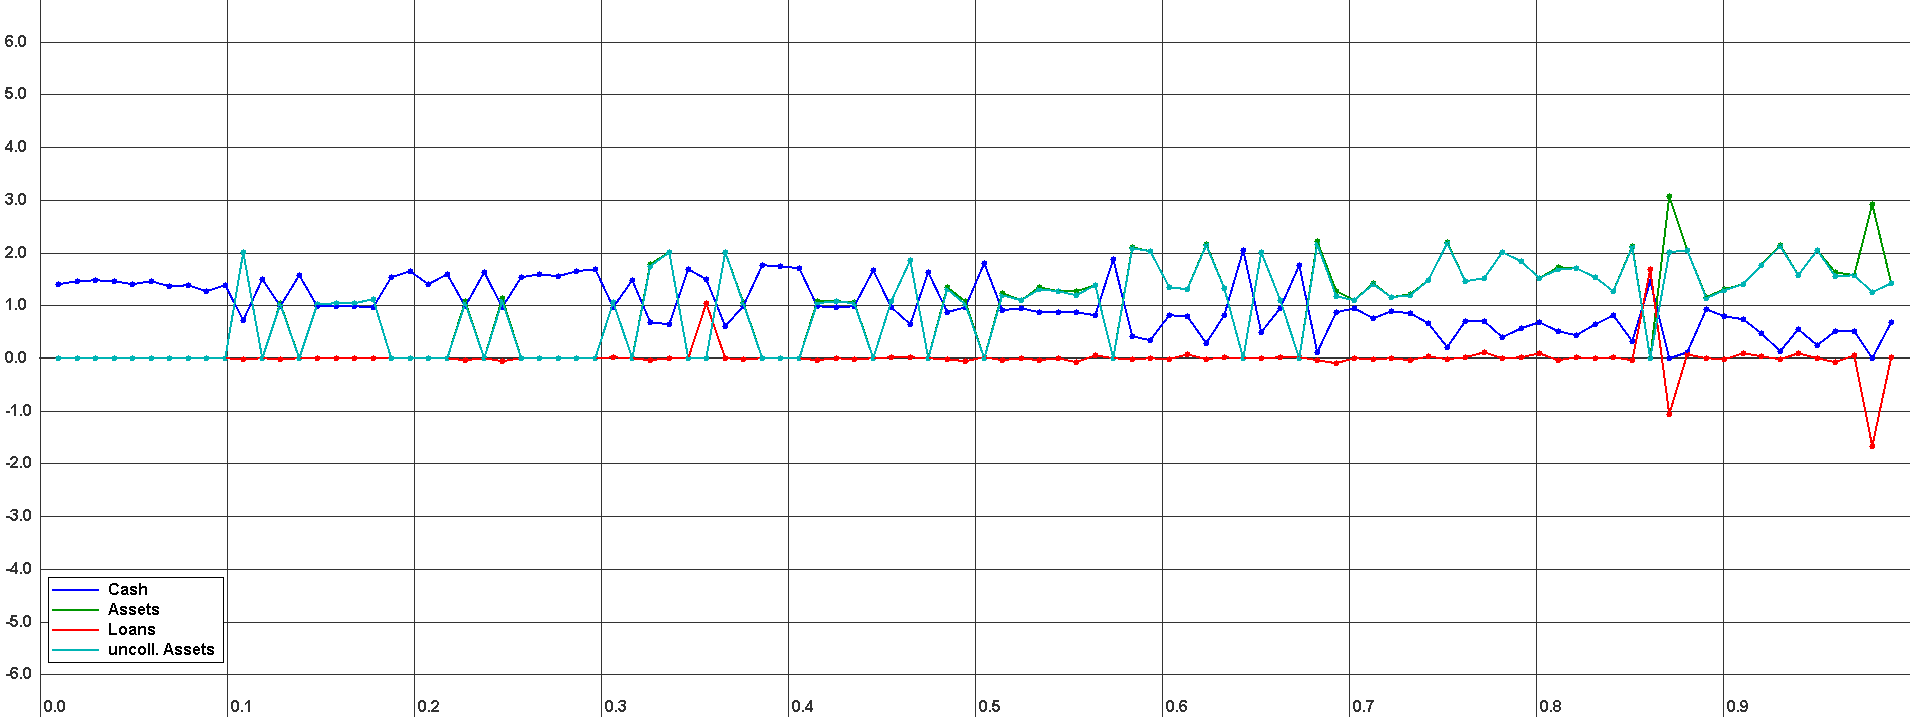
\includegraphics[width=1.0\textwidth, angle=0]{BARBASIALBERT_m03_m1_100_NOCOLLATERALMARKET_REPL.png}
	\caption{Wealth-Distribution of Barbasi-Albert m0=3, m=1 topology}
	\label{fig:wealth_BARBASIALBERT_m03_m1_100_NOCOLLATERALMARKET_REPL}
\end{figure}

need to show network too because random ?

\begin{figure}[H]
	\centering
  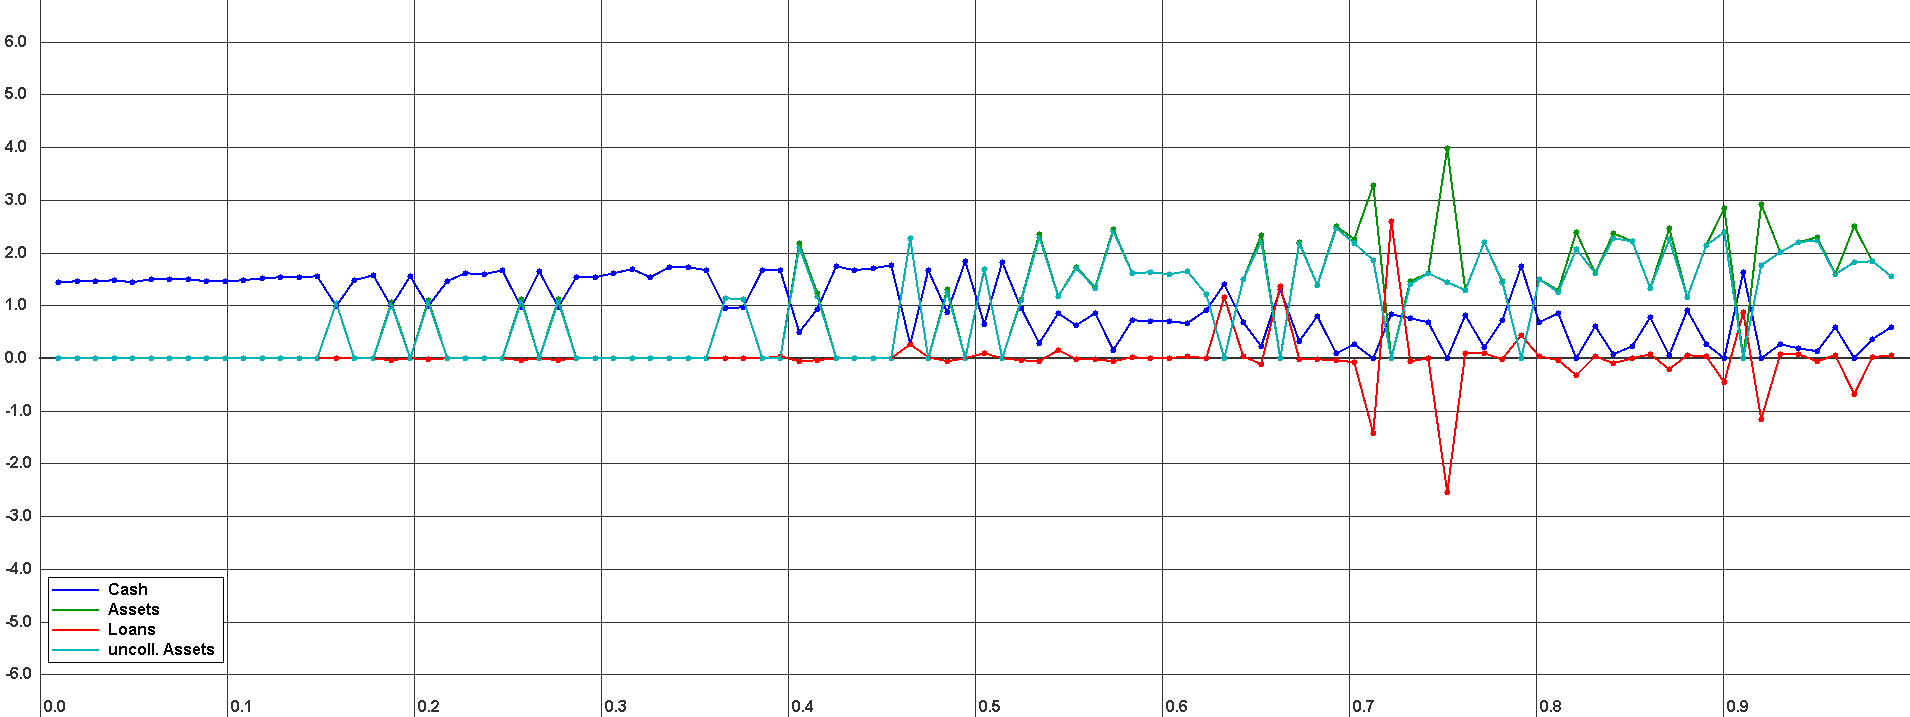
\includegraphics[width=1.0\textwidth, angle=0]{BARBASIALBERT_m09_m3_100_NOCOLLATERALMARKET_REPL.png}
	\caption{Wealth-Distribution of Barbasi-Albert m0=9, m=3 topology}
	\label{fig:wealth_BARBASIALBERT_m09_m3_100_NOCOLLATERALMARKET_REPL}
\end{figure}

need to show network too because random ?

\subsection{Watts-Strogatz}
todo: kann hypothese erfüllen mit entsprechender parameterisierung

\begin{figure}[H]
	\centering
  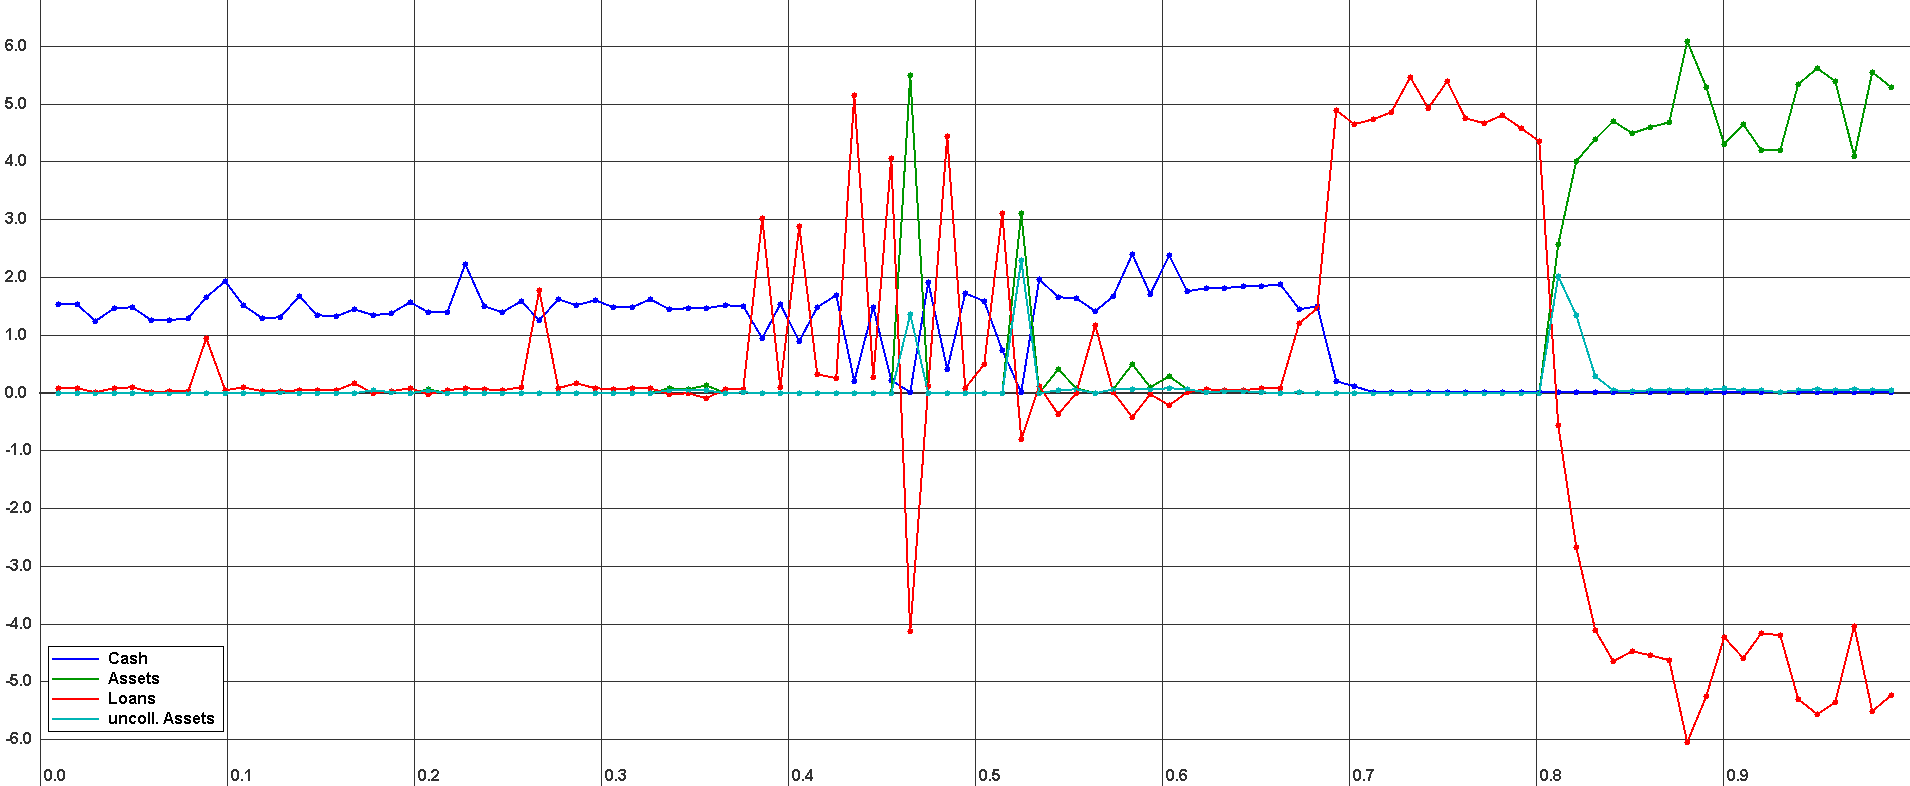
\includegraphics[width=1.0\textwidth, angle=0]{WATTSSTROGATZ_k2_b02_100_NOCOLLATERALMARKET_REPL.png}
	\caption{Wealth-Distribution of Watts-Strogatz k=2, b=0.2 topology}
	\label{fig:wealth_WATTSSTROGATZ_k2_b02_100_NOCOLLATERALMARKET_REPL}
\end{figure}

need to show network too because random ?

\end{document}
